\documentclass{article}

% ———————————————————————————————————————————————————————
%  PACKAGES (1 seule fois chacun)
% ———————————————————————————————————————————————————————
\usepackage{geometry}
\geometry{a4paper,left=0.6cm,right=0.7cm,top=1cm,bottom=1cm,columnsep=0.8cm}

\usepackage{times}
\usepackage{paracol}
\usepackage{enumitem}
\usepackage{fontawesome}
\usepackage{tabularx}
\usepackage{tikz}
\usepackage{adjustbox}
\usepackage[hidelinks]{hyperref}
\usepackage{xcolor}
\usepackage{ragged2e}

\setlist[itemize]{itemsep=2pt,topsep=0pt,leftmargin=*}
\renewcommand{\labelitemi}{\textcolor{maincolor}{$\bullet$}}

\newcolumntype{Y}{>{\RaggedRight\arraybackslash}X}
\setlength{\parindent}{0pt}

% ———————————————————————————————————————————————————————
%  COULEURS & MISE EN PAGE
% ———————————————————————————————————————————————————————
\definecolor{maincolor}{HTML}{2AAEE7}
\definecolor{lightgray}{HTML}{A0A0A0}

% bande colorée à droite
\usepackage{eso-pic}
\AddToShipoutPictureBG{%
  \begin{tikzpicture}[remember picture,overlay]
    \fill[maincolor!10] (0.7\paperwidth,0) rectangle (\paperwidth,\paperheight);
  \end{tikzpicture}
}

% en-tête de section compact
\newcommand{\cvsection}[1]{%
  \par\bigskip
  {\Large\bfseries #1}\par
  \noindent\rule{\linewidth}{0.6pt}\par
  \medskip
}

% ———————————————————————————————————————————————————————
%  DOCUMENT
% ———————————————————————————————————————————————————————
\begin{document}\pagestyle{empty}
\columnratio{0.7}\begin{paracol}{2}

% ========== Colonne principale ====================================
{\LARGE\bfseries Pape Saliou FALL}

{\color{maincolor}\Large\bfseries Ingénieur Data Scientist \& Développeur IA}

\medskip
%----------- contact résumé ----------------------------------------
\begin{tabular}{@{}cp{0.45\linewidth}}
  \color{maincolor}\faEnvelope & \href{mailto:papesalioufall2@gmail.com}{papesalioufall2@gmail.com}\\
  \color{maincolor}\faPhone    & \href{tel:07 53 48 14 53}{07 53 48 14 53}\\
  \color{maincolor}\faMapMarker& 95300 Pontoise\;\\
  \color{maincolor}\faLinkedin & \href{linkedin.com/in/pape-saliou-fall-43154a211}{pape-saliou-fall-43154a211}\\
\end{tabular}

\cvsection{PROFIL}
Data scientist confirmé, je transforme des ensembles de données complexes en solutions opérationnelles à forte valeur ajoutée. Formé à la Sorbonne et actif en CDI, j’exploite le machine learning, le deep learning et le cloud pour déployer des applications innovantes. Autonome, curieux et orienté résultats, j’apprécie le travail d’équipe et la culture du partage. Mon ambition : relever de nouveaux défis au sein d’un environnement qui mise sur l’innovation et l’excellence.

\cvsection{EXPÉRIENCE}

\colorbox{maincolor}{%
  \begin{minipage}{\linewidth}
    \textbf{Data Scientist \& Développeur IA} \\ Prepaya, Paris \\ 01/2024 – Présent
    \begin{itemize}
      \item Conçu et déployé une plateforme IA full-stack (Python/JavaScript) hébergée sur Heroku. \item Implémenté des modèles de machine \& deep learning pour l’analyse de séries chronologiques. \item Intégré l’API OpenAI et une base PostgreSQL afin d’automatiser les recommandations issues des données.
    \end{itemize}
  \end{minipage}}

\vspace{3mm}


\colorbox{maincolor}{%
  \begin{minipage}{\linewidth}
    \textbf{Apprenti Risk Analyst \& Data Scientist} \\ AXA XL (Groupe AXA), Paris \\ 12/2022 – 12/2023
    \begin{itemize}
      \item Automatisé la collecte des données financières avec Python/VBA, fiabilisant les rapports mensuels. \item Développé des tableaux de bord Power BI pour la facturation, améliorant la visibilité des KPI pour la direction. \item Créé des applications prédictives sur les sinistres (Python, R Shiny) pour estimer la probabilité d’occurrence.
    \end{itemize}
  \end{minipage}}

\vspace{3mm}


\colorbox{maincolor}{%
  \begin{minipage}{\linewidth}
    \textbf{Apprenti Data Scientist} \\ Prepaya, Paris \\ 09/2021 – 08/2022
    \begin{itemize}
      \item Appliqué le deep learning NLP (T5, BERT) pour générer automatiquement des formulaires clients. \item Réalisé des analyses de sentiment sur les avis clients afin d’orienter les actions marketing. \item Automatisé la collecte web (BeautifulSoup, Selenium) et documenté le code sous VS Code et LaTeX.
    \end{itemize}
  \end{minipage}}   %← généré par build_placeholders()

\cvsection{FORMATION}

    \begin{tabularx}{\linewidth}{@{}c X@{}}
    \textcolor{sidetext}{\faGraduationCap} &
    \textbf{Master 2 Data Science} \\
    & Sorbonne Université, Paris \\
    & \begin{itemize}[leftmargin=*]
  \item Statistique avancée, machine learning et deep learning appliqués aux grands ensembles de données. \item Analyse de séries temporelles, bases de données relationnelles et calcul parallèle. \item Conception et évaluation de modèles prédictifs pour la science des données.
\end{itemize} \\
    & \textit{09/2021 – 03/2022}
    \end{tabularx}
    

% ———— Colonne de droite (bleue) ————————————————
\switchcolumn
\color{black}           % le fond est déjà maincolor!10

\centering
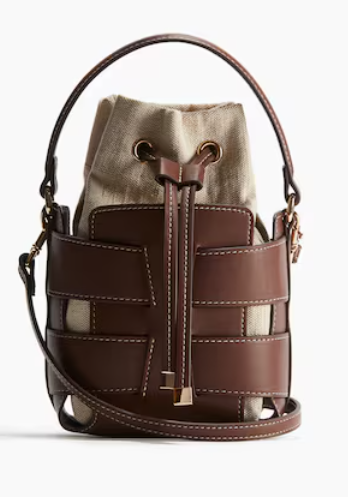
\includegraphics[width=3cm]{ff6cf73873a042d88cc0a8c3a23c0236.png}

\bigskip

\cvsection{COMPÉTENCES}

\begin{itemize}[leftmargin=*]
\item Python
\item JavaScript
\item C++
\item SQL
\item PowerBI
\item Git
\item Tensorflow\end{itemize}


\cvsection{LANGUES}

\begin{itemize}[leftmargin=*]
\item Français - \textcolor{gray}{Maternel}
\item Anglais - \textcolor{gray}{B2}\end{itemize}


\cvsection{CENTRES D’INTÉRÊT}

\begin{itemize}[leftmargin=*]
\item Football
\item Natation
\item Lecture
\end{itemize}


\end{paracol}
\end{document}
